\section{Introduction}
\label{sect:introduction}

Saeid

Supersymmetry \cite{Martin:1997ns} (SUSY) is one of the most promising extensions of the 
Standard Model of the elementary particles (SM) which solves both the 
quadratic divergencies and hierarchy problems simultaneously. It introduces a new symmetry between the bosons and fermions and 
for every particle a sparticle is defined which is exactly the same, but differ in spin by 1/2. 
%Since the super particles are not discovered yet, the supersymmetry should be a broken symmetry. 
%Various mechanisms are introduced to break the symmetry softly without changing the other interesting features of the theory.

In a hadron collider, like LHC, it is expected to see the signature of the colored SUSY partners, 
but the very extensive search in the LHC experiments pushes the mass of the colored particles much 
beyond the previous expectations. 
Looking at other sectors of the SUSY, e.g, electroweak production of the sparticles, is motivated not to miss SUSY in a corner.
A search for new physics using 20 \invfb of data from CMS taken in 2012 is documented in this note. 
Although the search is sensitive to any high scale 
new physics with a missing transverse momentum, an R-parity conserving SUSY model is used 
to illustrate the performance of the method.

Due to the special role of the third generation of the sparticles, events with two taus in the final state 
accompanying with the missing transverse energy (\met) are considered.
The two taus can be generated in the cascade of the staus or charginos:
\begin{linenomath}
\begin{equation}
p + p \rightarrow \tilde{\chi_{1}^{+}} + \tilde{\chi_{1}^{-}} ~~\mathrm{or}~~  p + p \rightarrow \tilde{\tau} + \tilde{\tau}
\end{equation}
\end{linenomath}
when 
\begin{linenomath}
\begin{equation}
\tilde{\chi_{1}^{+}} \rightarrow \tilde{\tau} + \nu ~~\mathrm{or}~~  \tilde{\chi_{1}^{+}} \rightarrow \tilde{\nu}_{\tau} + \tau 
\end{equation}
\end{linenomath}
and 
\begin{linenomath}
\begin{equation}
\tilde{\tau} \rightarrow \tau + \tilde{\chi_{1}^{0}} ~~\mathrm{or}~~  \tilde{\nu}_{\tau} \rightarrow \nu + \tilde{\chi_{1}^{0}} 
\end{equation}
\end{linenomath}
and $\tilde{\chi_{1}^{0}}$ can not be detected and appears as missing transverse momentum (\met).
In this note, we mainly focus on the $\tilde{\chi_{1}^{+}}\tilde{\chi_{1}^{-}}$ production which has a higher 
production cross section. Figure \ref{fig:Productions} shows our favorite decays.

\begin{figure}[!htb]
\centering
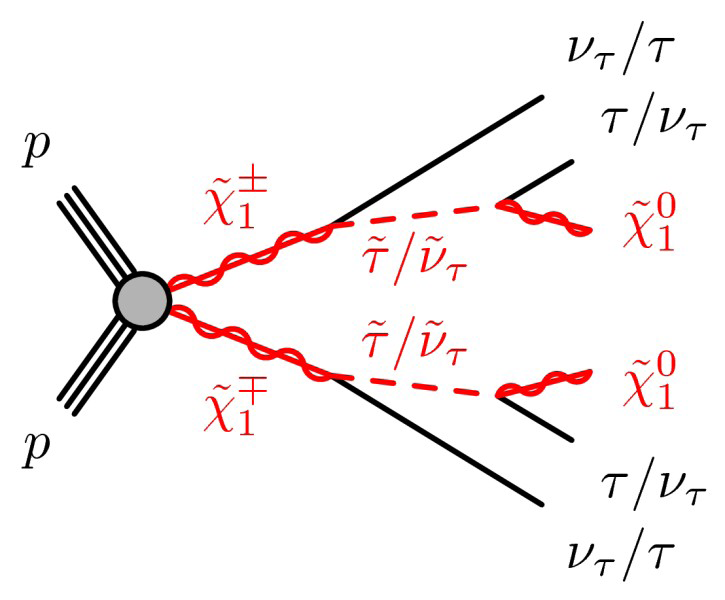
\includegraphics[width=0.49\textwidth]{Introductionfigs/DiChargino.png}
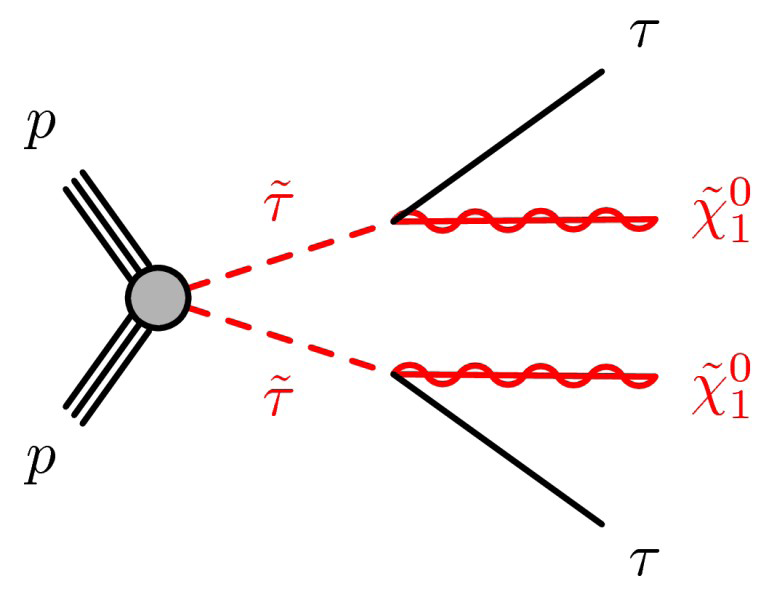
\includegraphics[width=0.49\textwidth]{Introductionfigs/DiSTau.png}
\caption{Schematic production of double tau from chargino pair and stau pair.}
\label{fig:Productions}
\end{figure}


The search variable is the stransverse mass (\mttwo) which is the natural extension of the known transverse mass (\mt) to a case 
when two massive particles with equal mass are created in pairs and decay via a chain of jets and leptons to two 
invisible particles. 
In the case of R-Parity conserving SUSY, the Lightest Supersymmetric Particle (LSP) escapes the detection and appears as 
a missing transverse momentum.
The distribution of \mttwo reflects the scale of the produced particles and is much higher for sparticles
compared to the SM particles. Hence, SUSY should appear as an excess in the tail of the \mttwo distribution.
It was shown previously \cite{MT2_2011} that \mttwo is a powerful variable to search for SUSY. 


After introduction in the next section the \mttwo variable is introduced. 




